\documentclass[a4paper, 12pt, oneside]{article}

\usepackage{float}
\usepackage{braket}

%Marges. Désactiver pour utiliser les valeurs LaTeX par défaut
%\usepackage[top=2.5cm, bottom=2cm, left=2cm, right=2cm, showframe]{geometry}
\usepackage[top=2.5cm, bottom=2cm, left=2cm, right=2cm]{geometry}

% quelques symboles mathematiques en plus
\usepackage{amsmath}
\usepackage{systeme}
\usepackage{multicol}
\usepackage{enumitem}
\usepackage{amssymb}

\usepackage{bm}
\usepackage{wrapfig}

\ProvidesPackage{gensymb}
[2022/10/13 v1.0.1 (KJH)]

\usepackage[font=small,labelfont=bf]{caption}
\usepackage{subcaption,graphicx}

\usepackage[T1]{fontenc}
\renewcommand{\familydefault}{\sfdefault}

\usepackage{xfrac}
\usepackage[utf8]{inputenc}

\usepackage[style=numeric-comp, sorting=none]{biblatex}
\addbibresource{report_citations.bib}

\usepackage[colorlinks,bookmarks=false,linkcolor=black,urlcolor=blue, citecolor=black]{hyperref}

\usepackage{units}

\usepackage{verbatim}
\usepackage{verbdef}% http://ctan.org/pkg/verbdef

\DeclareMathOperator*{\argmin}{argmin}
\makeatletter
\renewcommand{\section}{\@startsection{section}{1}{\z@}%
             {-3.5ex \@plus-1ex \@minus-.2ex}%
             {2.3ex \@plus.2ex}%
             {\normalfont\large\bfseries}}
\makeatother

\makeatletter
\renewcommand{\subsection}{\@startsection{subsection}{1}{\z@}%
             {-3.5ex \@plus-1ex \@minus-.2ex}%
             {2.3ex \@plus.2ex}%
             {\normalfont\normalsize\bfseries}}
\makeatother

\newcommand{\mail}[1]{{\href{mailto:#1}{#1}}}
\newcommand{\ftplink}[1]{{\href{ftp://#1}{#1}}}

% ======= The document begins here ======
\newcommand{\inlineeqnum}{\refstepcounter{equation}~~\mbox{(\theequation)}}
\begin{document}

\title{Semester Project: Variational Monte-Carlo for strongly correlated bosons in continuous space}
\author{Giorgio Facelli\\ 
{\small \mail{giorgio.facelli@epfl.ch}}}

\maketitle 
\begin{center}
Hosting group: CQSL lead by Prof.\ Giuseppe Carleo \\
Supervision: Gabriel Pescia
\end{center}

\baselineskip=16pt
\parindent=0pt
\parskip=12pt

\section{Introduction}
In recent years, tremendous improvements have been witnessed in the field of Machine Learning (ML) for science applications \cite{carleo_2019}. 
Many of these improvements have been triggered by the development of highly flexible and accurate architectures based on 
Artificial Neural Networks (ANNs) to approximate arbitrary high-dimensional functions, characteristic 
which gives to ANNs the notorious nickname {\it universal function approximators}. In particular, in the context of 
many-body quantum systems, symmetry-aware ANNs allowed the investigation of many-body wavefunctions by restricting 
considerably the ensemble of possible solutions. \\
Academic research fields such as condensed matter theory, quantum chemistry 
and materials science increasingly deal with many-body quantum systems, of which 
\textit{ab initio} analytical solutions often cannot be found because of their complex interactions.
Monte Carlo (MC) methods, at the expense of statistical errors, are good candidates for an exact 
description of the system. This family of techniques has in fact been shown to be very valuable in 
studying physical systems \cite{mcmillan_1965, schiff_1967,dornheim_2016, magro_1993, kroiss_2016}. 
One of them is the well-known {\it Variational Monte Carlo} (VMC), which introduces a variational 
ansatz that gets iteratively optimized until a minimum is found in energy, and the ground state 
wavefunction is found. However, recent research on the topics has shown that ANNs represent a 
promising candidate to solve some of these pressing problems. These methods generally work in 
conjuction with MC statistical techniques such as VMC.\\
Variational ansatzes parametrized by ANNs, often called Neural Quantum States (NQSs), can serve as optimal estimators of 
complicated and highly-entangled wavefunctions. Until now, many efforts have been devoted to study equilibrium 
and out-of-equilibrium systems with discrete degrees of freedom \cite{carleo_2017, hibat-allah_2020, choo_2018, 
choo_2020, czischek_2018, yoshioka_2021}. 
Quite recently, also early research work has developed state-of-the-art results for continuous-variable 
systems, both in periodic and non-periodic settings \cite{pescia_2022, pescia_2023, pfau_2020, hermann_2020}. \\
In this study, we implement a NQS architecture inspired from \textit{graph neural networks}, which can efficiently 
encode relationships in the data, called Message-Passing Neural Networks (MPNNs). We will apply this 
to study bosonic many-body quantum systems interacting through a gaussian core potential and with 
periodic boundary conditions (PBCs). In the Methods 
section we present the theoretical framework which allows to model the system, 
as well as the architecture employed as the ground-state variational ansatz. In the Results section, 
we first benchmark some important hyperparameters related to the ansatz. We then move on to study the 
physical properties of the system, where we show the presence of two distinct phases of matter. We 
then discuss the main results presented and finally draw the conclusions of this study.

\section{Methods}\label{sec:methods}

\subsection{Variational Monte carlo}\label{sec:var_principle}
The core idea of VMC is to exploit the {\it variational principle} to study the low-energy 
properties of many-body quantum systems. The principle states that the energy of a physical system is minimized 
by the ground state eigenvector $\ket{\Psi_0}$ associated to the Hamiltonian of the system:
\begin{equation}
    \ket{\Psi_0} = \argmin_{\ket{\Psi}} \Biggr[\dfrac{\braket{\Psi|\hat{H}|\Psi}}{\braket{\Psi|\Psi}}\Biggr]
\end{equation}
To do this, in VMC a variational ansatz $\ket{\Psi(\bm{\theta})}$ is used, and its parameters $\bm{\theta}$ are 
iteratively optimized so as to reach 
the minimum in energy. Hence, the estimator of the ground-state eigenvector will be $\ket{\Psi(\bm{\theta}_0)}$ such that $\bm{\theta}_0$ 
satisfies:
\begin{equation}
    \bm{\theta_0} = \argmin_{\bm{\theta}}\Biggr[\dfrac{\braket{\Psi(\bm{\theta})|\hat{H}|\Psi(\bm{\theta})}}
    {\braket{\Psi(\bm{\theta})|\Psi(\bm{\theta})}}\Biggr]
\end{equation}
This allows the variational ansatz to approximate the ground-state
eigenvector, with which we can gain insight to the physical properties of the 
system. 

\subsection{Estimation of observables}
Expectation values of observables cannot in general 
be computed efficiently. In fact, for $\braket{\hat{O}} = \braket{\Psi|\hat{O}|\Psi}/\braket{\Psi|\Psi}$, 
computing the normalization term is in general unfeasible. However, using MC integration, we can efficiently 
approximate most physical observables by a statistical average over its so-called \textit{local} observable:
\begin{equation}\label{eq:est_obs}
    \begin{split}
    \dfrac{\braket{\Psi|\hat{O}|\Psi}}{\braket{\Psi|\Psi}} &= 
    \dfrac{\int \,d\bm{x} \int \,d\bm{x'}\Psi(\bm{x})^*\braket{\bm{x}|\hat{O}|\bm{x}'}\Psi(\bm{x}')}{\int \,d\bm{x} |\Psi(\bm{x})|^2} = \\
    &= \dfrac{\int \,d\bm{x} |\Psi(\bm{x})|^2 O_{\text{loc}}(\bm{x})}{\int \,d\bm{x} |\Psi(\bm{x})|^2} = \mathbb{E}_{\Pi(\bm{x})}\biggr[O_{\text{loc}}(\bm{x})\biggr]
    \end{split}
\end{equation}

where we define $O_{\text{loc}}(\bm{x}) = \int \,d\bm{x'} O_{\bm{x}\bm{x}'} \frac{\Psi(\bm{x}')}{\Psi(\bm{x})}$ 
(and $O_{\bm{x}\bm{x}'} = \braket{\bm{x}|\hat{O}|\bm{x}'}$) and the expectation value after the last equality 
in Eq. (\ref{eq:est_obs}) is over the probability ditribution 
$\Pi(\bm{x}) = \frac{|\Psi(\bm{x})|^2}{\int \,d\bm{y} |\Psi(\bm{y})|^2}$. Finally,
by sampling a large enough set of samples $\{\bm{x}^{(i)}\}_{i=1}^M$ from $\Pi(\bm{x})$, one can 
approximate the observable:
\begin{equation}
    \braket{\hat{O}} = \frac{1}{M}\sum_{i=1}^M O_{\text{loc}}(\bm{x}^{(i)})
\end{equation}
The standard procedure of VMC is then to sample positions from the distribution given by the variational 
ansatz, estimate the mean energy and its gradient and then optimize the parameters in the direction of steepest 
descent, with the goal to minimize the mean energy. Many techniques can be used to generate a set of samples. In 
this work, we use the very well-known Metropolis-Hastings algorithm.

\subsection{Implementation of a periodic system}\label{sec:PBCs}
Periodic boundary conditions (PBCs) allow to access the bulk properties of 
extended systems. To be able to include PBCs in a given system, one must ensure 
that the wavefunction be invariant under translation of a single-particle position by a quantity corresponding to 
the simulation lattice vectors.
$\bm{x}_i \leftrightarrow \bm{x}_i+\bm{L}\cdot\bm{e}_k$ where $\bm{x}_i \in \mathbb{R}^d$ is the position of one particle 
in $d$ spatial dimensions, $\bm{L}$ is the simulation box size and $\bm{e}_k$ an arbitrary basis vector of the simulation 
cell. In order to ensure this condition, the particle positions are mapped into quasi-particle 
positions as follows: 
\begin{equation}
    \bm{x}_i \longmapsto \bm{r}_i=\Biggr(\sin\biggr(\dfrac{2\pi}{\bm{L}}\bm{x}_i\biggr), \cos\biggr(\dfrac{2\pi}{\bm{L}}\bm{x}_i\biggr)\Biggr)
\end{equation}
where $\sin(\frac{2\pi}{\bm{L}}\bm{x}_i) = (\sin(\frac{2\pi }{L_1}x_{i,1}),\ldots,\sin(\frac{2\pi}{L_d} x_{i,d}))$. Thus, 
the transformed position space will double in dimensionality, namely $\bm{r}_i \in \mathbb{R}^{2d}$. Similarly, one needs to respect the intrinsic 
periodicity of the system also when computing the inter-particle distances. Hence, in the variational ansatz we will consider a continuous version 
(for differentiation purposes) of the 
periodic inter-particle distance defined by $d_{\sin}(i,j) = \lVert \sin\left(\frac{\pi}{\bm{L}}\bm{x}_{ij}\right)\rVert$, where $\bm{x}_{ij} = \bm{x_i}-\bm{x_j}$.
Finally, to compute the euclidean distance between two particles, respecting also the PBCs, we use the \textit{minum image} convention:

\begin{equation}
    d(i,j) = \biggr\lVert \bm{x}_i -\bm{x}_j - \bm{L}\left\lfloor \dfrac{\bm{x}_i -\bm{x}_j}{\bm{L}}\right\rceil \biggr\rVert
\end{equation}

\subsection{Gaussian cores}\label{sec:gaussian_cores}
In this study, we consider a 2D system of Bose particles of spin zero interacting via a repulsive Gaussian-core potential, and in a simulation 
cell with with PBCs. The Hamiltonian 
takes the following form: 
\begin{equation}
    H = T+V = -\dfrac{\hbar^2}{2m}\sum_{i=1}^N \vec{\nabla}^2_{i} +  \varepsilon\sum_{i < j}^N \exp\left(-\dfrac{d(i,j)^2}{2\sigma^2}\right)
\end{equation}
Where $T$ and $V$ are the kinetic and potential energy respectively, $d(i,j)$ is the minimum image distance 
between two particles and $\varepsilon, \sigma$ are two constants.
This can be written in a more compact form by normalizing the particle positions by $\sigma^2$ and 
defining the quantum coupling constant $\Lambda = \frac{\hbar^2}{m\varepsilon\sigma^2}$:
\begin{equation}
H = - \dfrac{\Lambda}{2} \sum_{i=1}^N \vec{\nabla}^2_{i} + \sum_{i < j}^N \exp\left(-\dfrac{d(i,j)^2}{2}\right)
\end{equation}
Previous studies have shown that this system exhibits superfluid and crystalline quantum phases 
of matter depending on the quantum coupling constant $\Lambda$ and the density $\rho = \frac{N}{L^2}$ (or equivalently the 
average inter-particle distance $r_s = (\rho\sigma^2)^{-1/2}$) \cite{pescia_2022, kroiss_2016}. Here, 
we will investigate these phenomena by means of the MPNN architecture as described in the next section.


\subsection{Message-passing Neural Networks}\label{sec:methods_MPNN}
\begin{wrapfigure}[16]{r}{0.45\textwidth}
    %\vspace{-1.0cm}
    \centering
    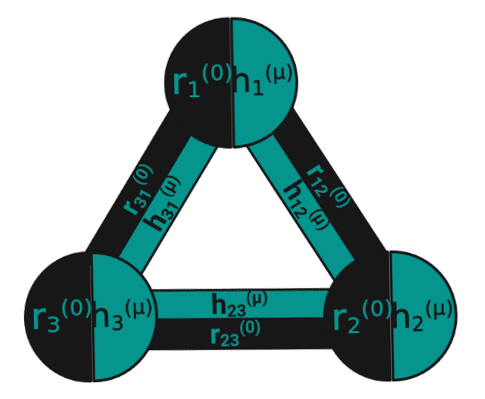
\includegraphics[scale=0.35]{figures/GNN_diagram.png}
    \captionsetup{width=0.35\textwidth} 
    \caption{\label{fig:GNN_diagram} Schematic representation of the $\mu$-th graph of a MPNN. In this case,
     three input coordinates $r_i^{(0)}$ generate three sets of distances $r_{ij}^{(0)}$, hidden nodes $h_{i}^{(\mu)}$ and hidden edges $h_{ij}^{(\mu)}$.}
\end{wrapfigure}

We propose here to use, as a variational ansatz, a family of graph neural networks (GNNs) known as 
message-passing neural networks (MPNNs). Their structure is schematically represented by a composition of graphs, such 
as the one depicted in Fig. \ref{fig:GNN_diagram}. These architectures have been shown 
to be well suited in processing data that can be represented as graphs \cite{scarselli_2009, micheli_2009}. In fact, their structure can encode information specific to each 
component in what are called \textit{nodes}, and information about their relationship, in what are 
known as \textit{edges}. In our context, information about the inter-particle distances is relevant in determining 
the spatial structure of the system. Hence, we will use the the edges to encode information 
about their interactions, and nodes to encode information about their positions. Briefly, for 
a MPNN with $\mathcal{N}$ graphs, $\mu$-th graph will have the following nodes and edges:

\begin{equation}
    \bm{n}_i^{(\mu)} = \biggr(\bm{r}_i, \bm{h}_i^{(\mu)}\biggr), \hspace{0.5cm} \bm{e}_{ij}^{(\mu)} = \biggr(\bm{r}_{ij},d_{\sin}(i,j), \bm{h}_{ij}^{(\mu)}\biggr)
\end{equation}
where $\bm{r}_i$ are the periodic quasi-particle coordinates introduced in section \ref{sec:PBCs}. 
These definitions include $\bm{h}_i^{(\mu)}$ and $\bm{h}_{ij}^{(\mu)}$, known as {\it hidden} nodes 
and edges, respectively, and defined as:
\begin{equation}
\bm{h}_{i}^{(\mu)} = \bm{f}\biggr(\bm{n}_i^{(\mu-1)}, \sum_{i\neq j} \bm{m}_{ij}^{(\mu)}\biggr), \hspace{0.5cm} \bm{h}_{ij}^{(\mu)} = \bm{g} \biggr(\bm{e}_{ij}^{(\mu-1)}, \bm{m}_{ij}^{(\mu)}\biggr)
\end{equation}
where $\bm{m}_{ij}^{(\mu)} = \phi \big(\bm{e}_{ij}^{(\mu-1)}\big)$. The functions $\bm{f},\bm{g},\bm{\phi}$ are 
multi-layer perceptrons (MLPs). For the purpose of this study, we will always take the same activation function $\text{GELU}\big(\cdot\big)$ 
for all MLPs.
Invariance under exchange of particles is a native property in wavefunctions describing bosonic systems. This 
translates to having a permutation-equivariant MPNN, which is ensured by taking the same hidden nodes 
and edges for all particles. Hence, we construct a variational ansatz $\Psi_{\bm{\theta}}$ by 
transforming the input coordinates into backflow coordinates $\bm{\tilde{x}}_i =\text{MPNN}(\bm{x})_i = \bm{n}_i^{(\mathcal{N})}$ and applying a 
final MLP $\bm{\rho}$: 

\begin{equation}
    \log[\Psi_{\bm{\theta}}(\bm{x})] = \sum_{i}\bm{\rho}(\bm{\tilde{x}}_i)=
    \sum_{i}\bm{\rho}(\text{MPNN}(\bm{x})_{i})
\end{equation}

where $\bm{x} = (\bm{x}_1,...,\bm{x}_N)$ are the original single-particle coordinates.

\subsection{LayerNorm}\label{sec:sec_LN}
To improve training we apply the so-called \textit{LayerNorm} (LN).
This feature proposes to re-center and normalize the nodes of a neural network layer after application 
of the activation function. If $\bm{y}$ is the output of a given layer with width $W$, then LN will 
induce the following transformation:

\begin{equation}
\bm{y'} = \dfrac{\bm{y}-\mu}{\sigma},\hspace{0.5cm}\mu = \dfrac{1}{W} \sum_{i=1}^W y_i,\hspace{0.5cm}
\sigma = \sqrt{\dfrac{1}{W}\sum_{i=1}^W(y_i-\mu)^2}
\end{equation}

This normalization has been shown to improve training for neural network models 
\cite{xu2019understanding}, with faster overall convergence. In a similar way, we will study the 
efficiency of this method on our optimizations and evaluate if it should be included in the definition 
of our MPNN model.

\subsection{Radial correlation function}
An important physical quantity to study the spatial structure among the simulated particles is the two-body radial correlation function. In short, this function tells us how 
likely a particle is going to be sitting at a distance $\bm{r}$ from a reference particle. It is defined as:
\begin{equation}\label{eq:rad_corr}
g_2(\bm{r}) = \dfrac{1}{N\rho}\braket{\sum_{i\neq j}^N\delta(\bm{r}-\bm{r}_{ij})}
\end{equation}
where $\delta(\cdot)$ is the delta function. The spherically averaged distribution is given by:
\begin{equation}\label{eq:pair_corr}
    g_2(r) = \dfrac{1}{N\rho}\dfrac{1}{4\pi r^2}\braket{\sum_{i\neq j}^N\delta(r-r_{ij})}
\end{equation} 
This is instead called the pair correlation function. Both the radial and pair correlation function will 
give us insight on the emergent physical structure of a system. 

\subsection{Structure factor}
Another important physical quantity is the structure factor, useful in determining the scattering 
properties of incident radiations on a material, which can be used to infer the atomic arrangement of a 
material. It relates the intensity of diffracted light as 
a function of the scattering vector $\bm{q} = \bm{k}_0 - \bm{k}_f$ (where $\bm{k}_0$ is the initial 
wavevector and $\bm{k}_f$ the final one). In mathematical terms:
\begin{equation}\label{eq:struct_factor}
    S(\bm{q}) = \dfrac{1}{N}\biggr|\braket{\sum_{i=1}^N e^{-i\bm{q} \cdot \bm{r}_i}}\biggr|^2
\end{equation}
where again $\bm{r}_i$ are the single-particle positions. In mathematical terms, the structure factor corresponds to the 
Fourier transform of the radial distribution function defined in Eq. (\ref{eq:rad_corr}):

\begin{equation}
    \begin{split}
    S(\bm{q}) &= \dfrac{1}{N}\biggr|\braket{\sum_{i=1}^N e^{-i\bm{q} \cdot \bm{r}_i}}\biggr|^2    
    = \dfrac{1}{N}\braket{\sum_{i,j}^N e^{-i\bm{q} \cdot (\bm{r}_i-\bm{r}_j)}} =
    1 + \dfrac{1}{N}\braket{\sum_{i\neq j}e^{-i\bm{q}(\bm{r}_i-\bm{r}_j)}} = \\ 
    &= 1 + \dfrac{1}{N}\braket{\int \,d\bm{r} e^{-i\bm{qr}} \sum_{i\neq j}\delta(\bm{r}-\bm{r}_i-\bm{r}_j)}  =
    1+\rho\int \,d\bm{r} e^{-i\bm{qr}} g_2(\bm{r})
    \end{split}
\end{equation}
where the last equality becomes straightforward by identifying $\bm{r}_i-\bm{r}_j = \bm{r}_{ij}$. 
\subsection{About the code}
The code has been entirely implemented on Python, with extensive use of libraries such as JAX, 
which allows automatic differentiation and just-in-time compilation, and Flax, a machine-learning library built 
specifically for JAX. Finally, the VMC approach, which includes sampling and optimization, is entirely automated through the NetKet library \cite{vicentini_2022}. 

\section{Results}\label{sec:results}
The results shown consider a system of $N=16$ bosons interacting via a 
gaussian-core potential. Unless said otherwise, the system is in a square simulation box and 
we set the quantum coupling constant $\Lambda = 1/30$. All simulations are conducted making use of 
\textit{stochastic gradient descent} and \textit{stochastic reconfiguration}. The latter computes the 
variational ansatz advanced infinitesimally in imaginary time, in order to maximize its overlap with the given variational ansatz 
at each optimization step. This step improves overall convergence, since an imaginary-evolved ansatz naturally tends 
to the ground state. In a first moment, we focus on the computational aspects of the architeture and its performance. Secondly, 
we investigate the physical aspects of the system, in particular phases of matter and ground-state properties.

\subsection{NQS architecture performances}

\subsubsection*{MPNN architecture}
Important features of the architecture are studied and their impact on the performance 
is investigated. In particular, we relate how the size of the architecture, and hence the number of 
parameters encoding the wavefunction, influences the precision of the ground-state approximation.
Considering the system at $\rho=1/9$, Fig. \ref{fig:fig_energy_vs_graphs} shows four energy optimizations, each with a different number of consecutive graphs, 
and similarly Fig. \ref{fig:fig_energy_vs_layers} with differing number of hidden layers in the $\bm{f},\bm{g},\bm{\phi}, \bm{\rho}$ MLPs as described in section \ref{sec:methods_MPNN}. In the first case, 
the number of graphs has a direct impact on the outcome of the simulation, resulting in increasingly 
better estimates of the ground-state energy. In the latter case, however, a high number of layers does 
not imply better performances. In Tab. \ref{tab:tab2} we report the values of final ground-state 
energies estimated during the optimizations reported in Figs. \ref{fig:fig_energy_vs_graphs}, \ref{fig:fig_energy_vs_layers},
where we note that the the number of graphs has a greater impact on the precision of the system'e energy.

\begin{table}[H]%[11]{r}{0.4\textwidth}
    \centering
    \caption{\label{tab:tab2} Ground-state energy per particle for $N=16$ at density $\rho= 1/9$ in 2D interacting through a 
    gaussian core potential, for different 
    number of graphs and different number of hidden layers.}
    \begin{tabular}{|c|c|c|}
        \hline
        n° &  graphs & hidden layers \\
        \hline
        \hline
        1 & $0.08515$ & $0.08516$ \\
        \hline
        2 & $0.08471$ & $0.08487$ \\
        \hline
        3 & $0.08468$ & $0.08471$ \\
        \hline
        4 & $0.08457$ & $0.08486$ \\
        \hline
    \end{tabular}
\end{table}

\begin{figure}[H]
    \begin{subfigure}{0.5\textwidth}
        \centering
        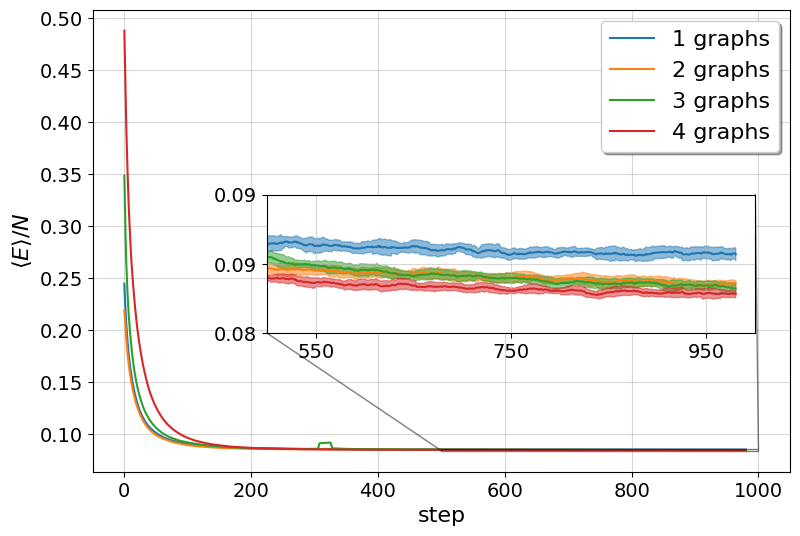
\includegraphics[width = 1.0\textwidth]{figures/energy_against_graphs.png}
            \caption{\label{fig:fig_energy_vs_graphs}}
    \end{subfigure}
    \begin{subfigure}{0.5\textwidth}
        \centering
        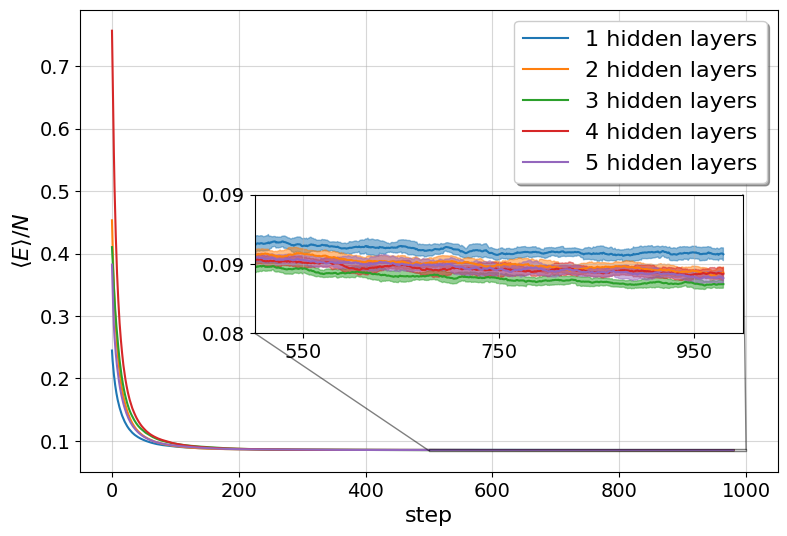
\includegraphics[width = 1.0\textwidth]{figures/energy_against_lyrs.png}
            \caption{\label{fig:fig_energy_vs_layers}}
    \end{subfigure}
    \caption{Comparison of energy optimizations for $N=16$ gaussian cores in 2D at $\rho=1/9$. \textbf{(a)} 
    Varying the number of graphs: the curves indicate that a better perfomance can be accessed with a greater number of graphs. 
    \textbf{(b)} Varying the number of hidden layers: here an increase in the variational parameters does not always increase accuracy 
    (optimization with $3$ hidden layers outperforms optimizations with $4$ or $5$).}
\end{figure}

\subsubsection*{LayerNorm} Here, we benchmark the performance of the additional normalization step 
LayerNorm as presented in section \ref{sec:sec_LN}. Multiple optimizations show that indeed LN is able to reach 
faster and precise convergence. In Tab. \ref{tab:tab_LN}, the energies per particle show that this method is able to reach 
lower values for the ground-state energies, yielding therefore more accurate results. Given the clear advantage of the LayerNorm 
additional step, the next results will make use of it.
\begin{table}[H]
    \centering
    \captionsetup{width=0.7\textwidth}
    \caption{\label{tab:tab_LN} Energy per particle for $\rho = 4/9, 1/9$ with and without applying LN after each activation 
    layer in the MPNN architecture.}
    \begin{tabular}{|c|c|c|}
        \hline
        & No \textbf{LN} & \textbf{LN} \\
        \hline
        \hline
        $\rho = 4/9$ & $1.00498$ & $1.00403$ \\
        \hline
        $\rho = 1/9$ &  $0.08534$ & $0.08515$ \\
        \hline
    \end{tabular}

\end{table}

\subsection{Quantum phases of matter}
To better understand the quantum phases of matter that the system has, we study the impact of the system density 
on the pair correlation function, defined as in Eq. (\ref{eq:pair_corr}), which gives us insight on how the position 
of one particle correlates to another one. To witness the structural changes, we take inspiration from 
the ground-state phase diagram in Ref. \cite{kroiss_2016} and consider $\rho=4/9,1/9,1/16$. Results are showed in 
Fig. \ref{fig:corr_func_diff_densities}, revealing two different phases of matter. 
In a first moment the high density yields a supefluid phase of matter (blue plot in the figure). At 
intermediate dentities, instead, the potential energy becomes more important and triangular 
crystalline phase arises. This is visible in green and especially orange plots, where their periodicity in the radial correlation function also at large distances arises because of long range order, which is 
indication of crystal structure.

\begin{figure}[H]
    \centering
    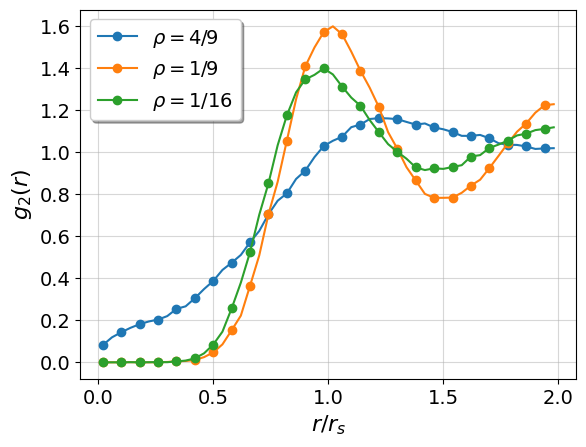
\includegraphics[scale = 0.6]{figures/corr_func_diff_densities.png}
    \caption{\label{fig:corr_func_diff_densities}Ground-state pair correlation function as a function of the normalized distance
    for $N=16$ gaussian cores in 2D at average densities of $4/9$ (blue), $1/9$  (orange), $1/16$ (green). The plots indicate 
    an initial liquid phase at high densitites with a non-zero value at the origin. At intermediate densities,
    a crystalline phase appears, showing a vanishing value of $g_2(r)$ at low distances and a periodic behaviour at higher 
    ones. Then, the oscillating structure weakens again for low densities. The final ground-state 
    energy-per-particle are $E/N = 1.00498, 0.08533, 0.02440$ respectively.}
\end{figure}

\subsection{Geometry of the simulation box and its impact on the system}
We now look at the influence of the system's geometry on the crystalline structure of the system. 
In particular, by changing the ratio of the simulation box by a factor $a$, yielding dimensions 
$\bm{L} = (L\sqrt{a}, L/\sqrt{a})$, we can gain insight on the impact that the aspect ratio has.
In this section, we consider $\Lambda = 1/100$ and $\rho=1/9$. This ensures that the 
system is well within the boundaries of the crystalline phase. Firstly, Fig. \ref{fig:gs_energy_diff_a} reports the 
ground-state energy as a function of the factor $a$, revealing a local minimum at $a=2/\sqrt{3}$. This 
is in fact the most natural configuration of the system, since the ratio is in accordance with that of the 
primitive lattice vectors, leading to a relaxation in energy. The aspect ratio $a$ has impact on the 
crystalline structure as well, increasing the magnitude of damping in the periodicity of the pair correlation function (see 
Fig. \ref{fig:corr_func_diff_a}).

\begin{figure}[H]
    \begin{subfigure}{0.5\textwidth}
        \centering
        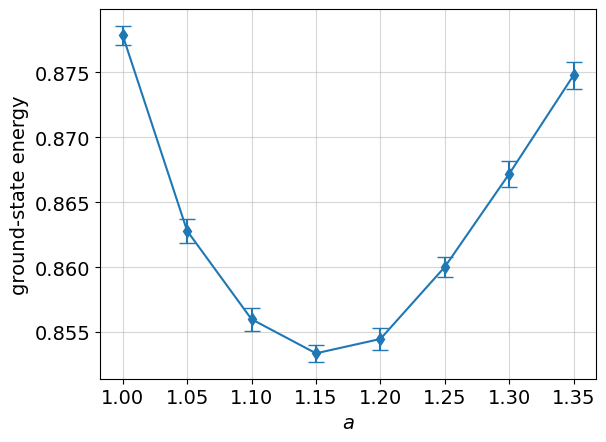
\includegraphics[width=1.0\textwidth]{figures/gs_energy_against_a_iters=2000.png}
        \caption{}
        \label{fig:gs_energy_diff_a}
    \end{subfigure}
    \begin{subfigure}{0.5\textwidth}
        \centering
        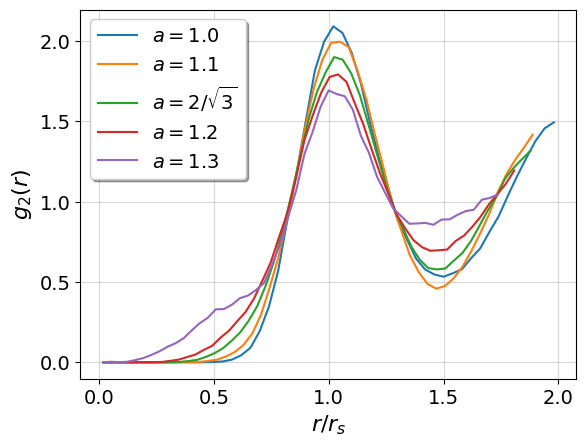
\includegraphics[width=1.0\textwidth]{figures/corr_func_diff_a_2.png}
        \caption{}
        \label{fig:corr_func_diff_a}
    \end{subfigure}
    \caption{System of $N=16$ particles in 2D at $\rho=1/9$, interacting though a gaussian-core potential \textbf{(a)} Total ground-state energy as a function of
    the aspect ratio $a$. A minimum is found in the vicinity of $a=\sqrt{2}/3$. All error bars are all $1\sigma$ away from the 
    mean. \textbf{(b)} Pair correlation function against the distance $r/r_s$, for different values of 
    $a$. A dampening effect is seen as $a$ is increased to higher values.}
\end{figure}

To gain a deeper understanding of the self-assembling arrangement of the system and the respective localization of its consituents,
we also plot in Figs. \ref{fig:corr_xy_diff_a}, \ref{fig:structure_factor_diff_a} the radial distribution function 
(Eq. (\ref{eq:rad_corr})) as well as the square root of the structure factor (Eq. (\ref{eq:struct_factor})) for different values 
of the aspect ratio, namely $a=1,1.1,\sqrt{2}/3,1.3$. In both sets of plots, the patterns indicate that for $a=2/\sqrt{3}$ the 
particles are in a more localized arrangement with respect to the other ones. In fact, for a simple square box ($a=1$), we only have a 
radial-dependent correlation, which breaks for $a > 1$ and we start to see well-localized clusters of 
high-probability occupation. The same can be said in regards to the structure factor, where $a=2/\sqrt{3}, 1.3$ are the ratios 
in which $S(\bm{q})$ is most localized.


\begin{figure}
    \begin{subfigure}{0.5\textwidth}
        \centering
        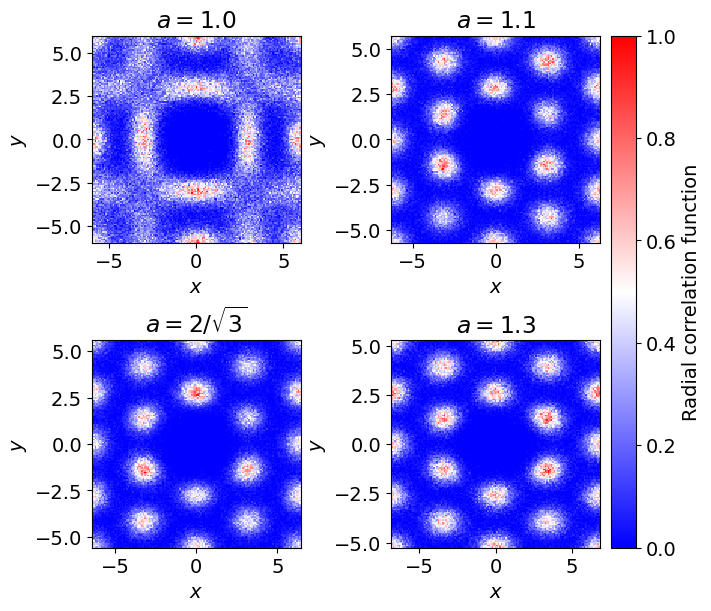
\includegraphics[width=1.0\textwidth]{figures/pair_corr_func_xy_diff_a_2.png}
        \caption{\label{fig:corr_xy_diff_a}}
    \end{subfigure}
    \begin{subfigure}{0.5\textwidth}
        \centering
        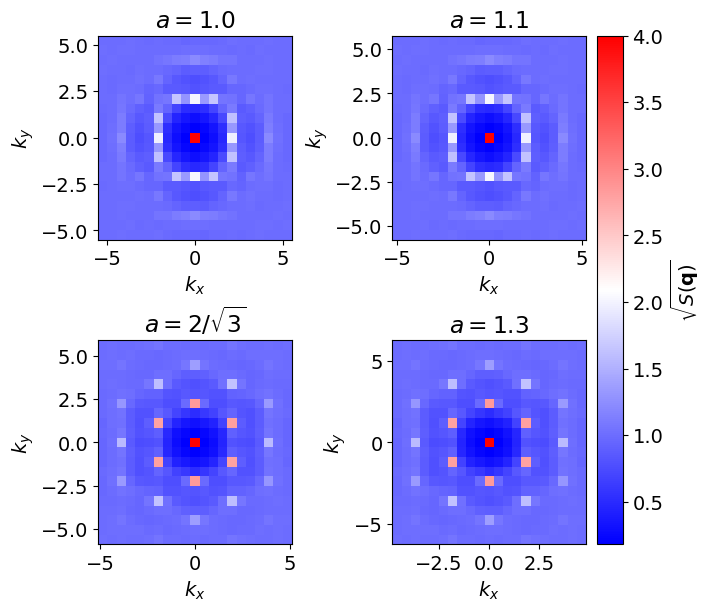
\includegraphics[width=1.0\textwidth]{figures/structure_factor_diff_a.png}
        \caption{\label{fig:structure_factor_diff_a}}
    \end{subfigure}
    \caption{System of $N=16$ particles at $\rho=1/9$ in 2D iteracting through a gaussian core potential.
    \textbf{(a)} Radial correlation function as a function of spatial coordinates $\bm{r} = (x,y)$, for different 
    values of the system's aspect ratio. \textbf{(b)} Square root of the structure factor as a function of the 
    wavevector $\bm{q} = (k_x, k_y)$, for different values of the system's aspect ratio. The $(\cdot)^{\frac{1}{2}}$ 
    rescaling allows to make the patterns more visible for each plot.}
\end{figure}

\section{Discussion}
In this study, the MPNN-based architecture has been put to the test by studying the ground-state 
properties of a 2D system of $N=16$ bosons interacting through a gaussian-core potential. We have shown good 
estimations of the ground-state energy, in line with results of similar systems in Ref. \cite{pescia_2022}. The approximations can be further improved by encoding the variational ansatz into a 
greater number of parameters. This can be achieved by tuning hyperparameters of the architecture 
such as number of graphs, number of layers and width of the layers. In particular, we have seen that 
increasing the number of graphs is the most effective hyperparameter, as it consistently improves the energy 
estimation. Instead, the number of hidden layers does not have a direct impact on the perfomance.
This is very likely due to a redundancy of the parameters, which does not always guarantee an improvement in the accuracy.  Moreover, the variational ansatz has proven to be versatile and able to encode the 
ground-state wavefunction in all scenarios which we considered, without any initial bias on the expected 
structure of the system. This allowed us also to study its physical properties, where it was shown 
that the system presents two different phases of matters, superfluid and crystalline, depending 
on the density. For high values of $\rho$ the 
dynamics of the system is completely dominated by quantum delocalization given the high-energy 
interactions. For low values, the system is instead relaxed as the potential energy is much smaller than the
energy of zero point fluctuations, and therefore the system cannot self-assemble into a crystal-like 
structure. At intermediate values of the density ($\rho=1/9$), there is instead good balance between 
the interaction and kinetic energy, which allows the system to organize into a triangular crystal phase.
Given that the solid phase has a triangular-like unit cell, we further studied the properties of the 
system for different aspect ratios $a$ of the simulation box. A relaxation in energy 
is seen until $a=2/\sqrt{3}$ (see Fig. \ref{fig:gs_energy_diff_a}). This is because it is the same 
aspect ratio as the primitive lattice vectors, and thus the box will be able to host more naturally 
the crystallization of the system. As a consequence, the radial correlation function in 
Fig. \ref{fig:corr_xy_diff_a} has more localized clusters of 
high-probability occupation, which represent the more robust crystalline structure of the system. 
Similarly, the structure factor (Fig. \ref{fig:structure_factor_diff_a}) has a greater quantization of 
wavevectors $\bm{q}$ allowed for scattering, reflecting the fact that the real-space lattice has a 
well-defined structure. It would be of interest to conduct the same studies on a larger system, and understand 
which results generalize well and which ones instead are caused by finite size effects.

\section{Conclusions}
In this study we presented novel state-of-the-art NQS architectures based on GNNs to study 
bosonic particles under a gaussian core interaction in a periodic system. The perfomance was 
investigated by varying the hyperparameters of the MPNN model, such as number of graphs and hidden 
layers. Its accuracy shows that indeed the model is able capture the behaviour of highly-correlated 
quantum systems. We then studied the ground-state properties, with particular 
emphasis on its phases of matter and the corresponding emergent structures. It was found that the system 
has a crystalline and superfluid phase, the latter emerging at higher or lower densities. 
The results were also in good agreement with similar studies that considered larger system sizes, 
such as Refs. \cite{pescia_2022, kroiss_2016}. Finally, just like done in Ref. \cite{pescia_2023}, it would be of 
great interest to extend such architectures to fermionic systems and test its performance when 
antisymmetric wavefunctions are considered. 
These advanced computational techniques pave the way to further research in the context of many-body 
quantum systems in continuous space, essential in disciplines such as quantum chemistry and 
materials science.

\printbibliography

\end{document}